\documentclass[ucs,9pt]{beamer}

% Copyright 2004 by Till Tantau <tantau@users.sourceforge.net>.
%
% In principle, this file can be redistributed and/or modified under
% the terms of the GNU Public License, version 2.
%
% However, this file is supposed to be a template to be modified
% for your own needs. For this reason, if you use this file as a
% template and not specifically distribute it as part of a another
% package/program, I grant the extra permission to freely copy and
% modify this file as you see fit and even to delete this copyright
% notice.
%
% Modified by Tobias G. Pfeiffer <tobias.pfeiffer@math.fu-berlin.de>
% to show usage of some features specific to the FU Berlin template.

% remove this line and the "ucs" option to the documentclass when your editor is not utf8-capable
\usepackage[utf8x]{inputenc}    % to make utf-8 input possible
\usepackage[german]{babel}     % hyphenation etc., alternatively use 'german' as parameter

% Template for talks using the Corporate Design of the Freie Universitaet
%   Berlin, created following the guidelines on www.fu-berlin.de/cd by
%   Tobias G. Pfeiffer, <tobias.pfeiffer@math.fu-berlin.de>
% This file can be redistributed and/or modified in any way you like.
%   If you feel you have done significant improvements to this template,
%   please consider providing your modified version to
%   https://www.mi.fu-berlin.de/w/Mi/BeamerTemplateCorporateDesign

\usepackage{amsmath,dsfont,listings}

%%% FU logo
% small version for upper right corner of normal pages
\pgfdeclareimage[height=0.9cm]{university-logo}{FULogo_RGB}
\logo{\pgfuseimage{university-logo}}
% large version for upper right corner of title page
\pgfdeclareimage[height=1.085cm]{big-university-logo}{FULogo_RGB}
\newcommand{\titleimage}[1]{\pgfdeclareimage[height=2.92cm]{title-image}{#1}}
\titlegraphic{\begin{center}\pgfuseimage{title-image}\end{center}}
%%% end FU logo

% NOTE: 1cm = 0.393 in = 28.346 pt;    1 pt = 1/72 in = 0.0352 cm
\setbeamersize{text margin right=3.5mm, text margin left=7.5mm}  % text margin

% colors to be used
\definecolor{text-grey}{rgb}{0.45, 0.45, 0.45} % grey text on white background
\definecolor{bg-grey}{rgb}{0.66, 0.65, 0.60} % grey background (for white text)
\definecolor{fu-blue}{RGB}{0, 51, 102} % blue text
\definecolor{fu-green}{RGB}{153, 204, 0} % green text
\definecolor{fu-red}{RGB}{204, 0, 0} % red text (used by \alert)

% switch off the sidebars
% TODO: loading \useoutertheme{sidebar} (which is maybe wanted) also inserts
%   a sidebar on title page (unwanted), also indents the page title (unwanted?),
%   and duplicates the navigation symbols (unwanted)
\setbeamersize{sidebar width left=0cm, sidebar width right=0mm}
\setbeamertemplate{sidebar right}{}
\setbeamertemplate{sidebar left}{}
%    XOR
% \useoutertheme{sidebar}

% frame title
% is truncated before logo and splits on two lines
% if neccessary (or manually using \\)
\setbeamertemplate{frametitle}{%
    \vskip-30pt \color{text-grey}\large%
    \begin{minipage}[b][23pt]{80.5mm}%
    \flushleft\insertframetitle%
    \end{minipage}%
}

%%% title page
% TODO: get rid of the navigation symbols on the title page.
%   actually, \frame[plain] *should* remove them...
\setbeamertemplate{title page}{
% upper right: FU logo
\vskip2pt\hfill\pgfuseimage{big-university-logo} \\
\vskip6pt\hskip3pt
% title image of the presentation
\begin{minipage}{11.6cm}
\hspace{-1mm}\inserttitlegraphic
\end{minipage}

% set the title and the author
\vskip14pt
\parbox[top][1.35cm][c]{11cm}{\color{text-grey}\inserttitle \\ \small \insertsubtitle}
\vskip11pt
\parbox[top][1.35cm][c]{11cm}{\small \insertauthor \\ \insertinstitute \\[3mm] \insertdate}
}
%%% end title page

%%% colors
\usecolortheme{lily}
\setbeamercolor*{normal text}{fg=black,bg=white}
\setbeamercolor*{alerted text}{fg=fu-red}
\setbeamercolor*{example text}{fg=fu-green}
\setbeamercolor*{structure}{fg=fu-blue}

\setbeamercolor*{block title}{fg=white,bg=black!50}
\setbeamercolor*{block title alerted}{fg=white,bg=black!50}
\setbeamercolor*{block title example}{fg=white,bg=black!50}

\setbeamercolor*{block body}{bg=black!10}
\setbeamercolor*{block body alerted}{bg=black!10}
\setbeamercolor*{block body example}{bg=black!10}

\setbeamercolor{bibliography entry author}{fg=fu-blue}
% TODO: this doesn't work at all:
\setbeamercolor{bibliography entry journal}{fg=text-grey}

\setbeamercolor{item}{fg=fu-blue}
\setbeamercolor{navigation symbols}{fg=text-grey,bg=bg-grey}
%%% end colors

%%% headline
\setbeamertemplate{headline}{
\vskip4pt\hfill\insertlogo\hspace{3.5mm} % logo on the right

\vskip6pt\color{fu-blue}\rule{\textwidth}{0.4pt} % horizontal line
}
%%% end headline

%%% footline
\newcommand{\footlinetext}{\insertshortinstitute, \insertshorttitle, \insertshortdate}
\setbeamertemplate{footline}{
\vskip5pt\color{fu-blue}\rule{\textwidth}{0.4pt}\\ % horizontal line
\vskip2pt
\makebox[123mm]{\hspace{7.5mm}
\color{fu-blue}\footlinetext
\hfill \raisebox{-1pt}{\usebeamertemplate***{navigation symbols}}
\hfill \insertframenumber}
\vskip4pt
}
%%% end footline
\usepackage{xcolor}
\definecolor{dkgreen}{rgb}{0,0.6,0}
\definecolor{gray}{rgb}{0.5,0.5,0.5}
\definecolor{mauve}{rgb}{0.58,0,0.82}
\definecolor{bgcolor}{HTML}{EDF0F2}
%%% settings for listings package
% \lstset{extendedchars=true, showstringspaces=false, basicstyle=\footnotesize\sffamily, tabsize=2, breaklines=true, breakindent=10pt, frame=l, columns=fullflexible}
\usepackage[scaled]{beramono}
\lstset{numbers=left,
	backgroundcolor=\color{bgcolor},
	numberstyle=\tiny,
	numbersep=5pt,
	breaklines=true,
	showstringspaces=false,
	frame=single,
	xleftmargin=15pt,
	xrightmargin=15pt,
	basicstyle=\ttfamily\scriptsize,
	stepnumber=1,
	keywordstyle=\color{blue},          % keyword style
  	commentstyle=\color{dkgreen},       % comment style
  	stringstyle=\color{mauve}         % string literal style
}
%Sprache Festelegen
% \lstset{language=R}
\lstset{language=C++} % this sets the syntax highlighting
\lstset{mathescape=true} % this switches on $...$ substitution in code
% enables UTF-8 in source code:
\lstset{literate={ä}{{\"a}}1 {ö}{{\"o}}1 {ü}{{\"u}}1 {Ä}{{\"A}}1 {Ö}{{\"O}}1 {Ü}{{\"U}}1 {ß}{\ss}1}
%%% end listings  % THIS is the line that includes the FU template!

\usepackage{arev,t1enc} % looks nicer than the standard sans-serif font
% if you experience problems, comment out the line above and change
% the documentclass option "9pt" to "10pt"

\usepackage{listings}

% image to be shown on the title page (without file extension, should be pdf or png)
\titleimage{title}

\title[SAMRAI vs. AMReX]{Ein Vergleich von SAMRAI und AMReX}

\author{Maikel Nadolski}

\institute[FU Berlin] % (optional, but mostly needed)
{Freie Universität Berlin}
% - Keep it simple, no one is interested in your street address.


% you can redefine the text shown in the footline. use a combination of
% \insertshortauthor, \insertshortinstitute, \insertshorttitle, \insertshortdate, ...
\renewcommand{\footlinetext}{\insertshortinstitute, \insertshorttitle}

% \addtobeamertemplate{navigation symbols}{}{%
%     \usebeamerfont{footline}%
%     \usebeamercolor[fg]{footline}%
%     \hspace{1em}%
%     \insertframenumber/\inserttotalframenumber
% }

% Delete this, if you do not want the table of contents to pop up at
% the beginning of each subsection:
\AtBeginSubsection[]
{
  \begin{frame}<beamer>{Übersicht}
    \tableofcontents[currentsection,currentsubsection]
  \end{frame}
}

\begin{document}

\begin{frame}[plain]
  \titlepage
\end{frame}

% \begin{frame}{Übersicht}
%   \tableofcontents
% \end{frame}

\begin{frame}{Daten Verwaltung}
\section {Daten Verwaltung}
Beide Bibliotheken haben überschneidende aber unterschiedliche Daten Verwaltung für die gleichen Konzepte.

\vspace{1cm}
\textbf{Dimensionalität}

\begin{center}
\begin{tabular}{l|l}
\texttt{SAMRAI\_MAXIMUM\_DIMENSION} & \texttt{AMREX\_SPACEDIM}
\end{tabular}
\end{center}
\end{frame}

\begin{frame}{Daten Verwaltung}
\textbf{Indexraum}

\vspace{1cm}
\begin{center}
\begin{tabular}{l|l}
\texttt{SAMRAI::hier::BlockId}      & \\
\hline
\texttt{SAMRAI::hier::Index}        & \texttt{amrex::IntVect}  \\
\hline
\texttt{SAMRAI::hier::IntVector}    & \\
\hline
                                    & \texttt{amrex::IndexType}\\
\hline
\texttt{SAMRAI::hier::Box}          & \texttt{amrex::Box}      \\
\hline
\texttt{SAMRAI::hier::BoxContainer} & \texttt{amrex::BoxArray} \\
\hline
\texttt{SAMRAI::hier::BoxLevel}     & \texttt{amrex::BoxArray} \\
                                    & + \texttt{amrex::DistributionMapping} \\
\end{tabular}
\end{center}
\end{frame}

\begin{frame}[fragile]{Polymorphe AMReX Boxen}
Boxen in \texttt{AMReX} sind in ihrem Indextyp polymorph.
\begin{center}
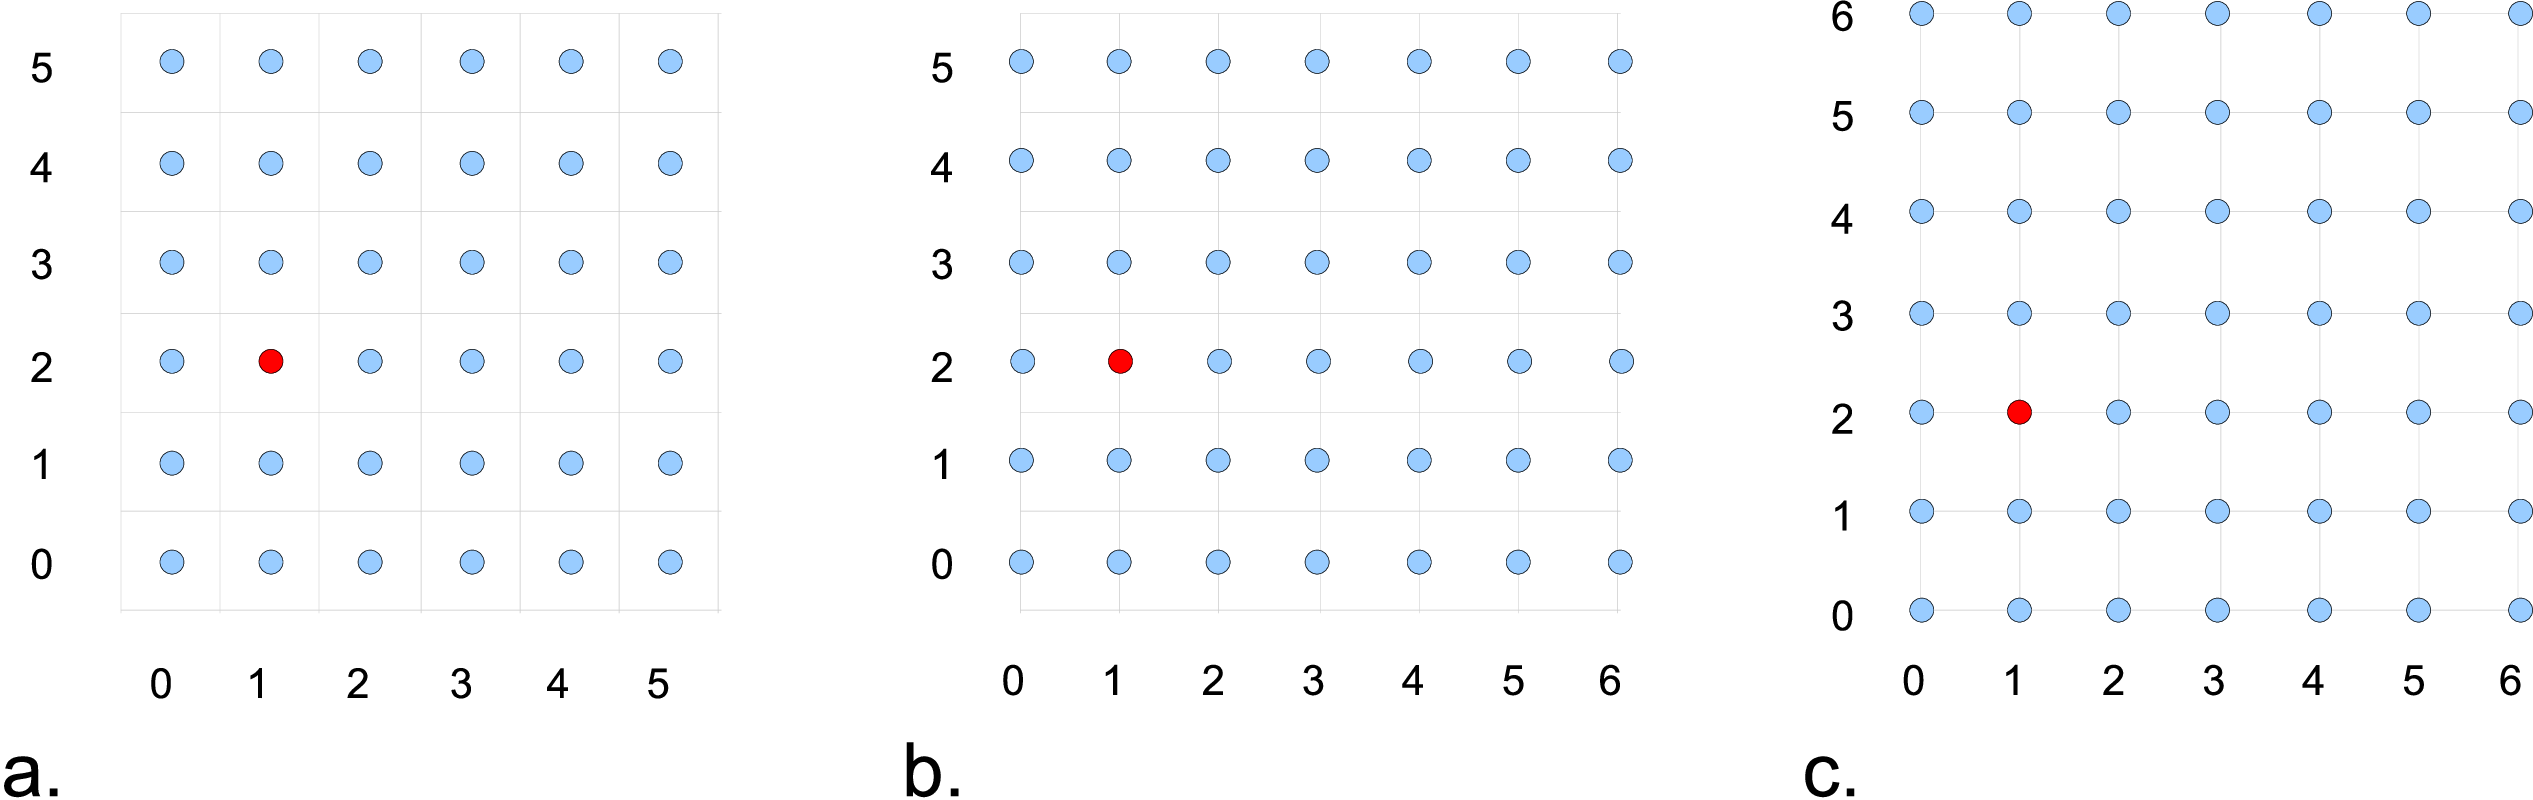
\includegraphics[width=0.5\textwidth]{indextypes}
\end{center}
\begin{lstlisting}
// By default, Box is cell-centered.
amrex::Box cell_box({0, 0}, {5, 5});
// Construct a face-centered Box with normal X direction 
amrex::Box face_box({0, 0}, {6, 5}, {1, 0});
// Construct a nodal Box.
amrex::Box node_box({0, 0}, {6, 6}, {1, 1});

// Conversion is possible
assert(amrex::convert(cell_box, {1, 0}) == face_box);
\end{lstlisting}
\pause
\vspace{0.4cm}
\emph{\texttt{SAMRAI::hier::Box} ist immer Zell-zentriert.}
\end{frame}

\begin{frame}{Daten Verwaltung}
\begin{center}
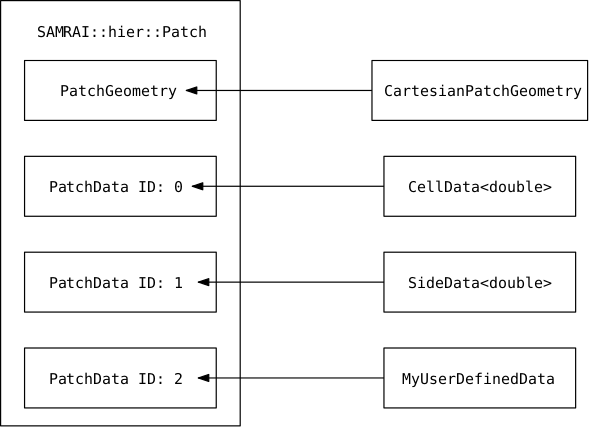
\includegraphics[width=0.8\textwidth]{patch}
\end{center}
\end{frame}

\begin{frame}{Daten Verwaltung}
\begin{center}
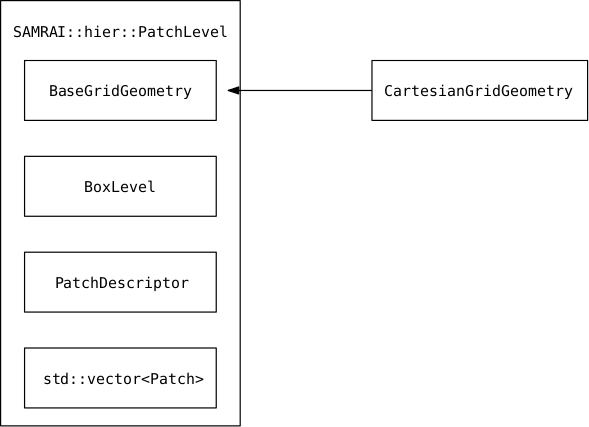
\includegraphics[width=0.8\textwidth]{patch_level}
\end{center}
\end{frame}

\begin{frame}{Daten Verwaltung}
\begin{center}
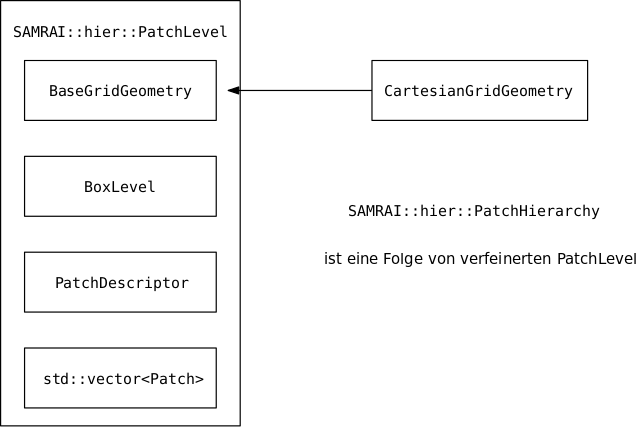
\includegraphics[width=0.8\textwidth]{patch_hierarchy}
\end{center}
\end{frame}

\begin{frame}{Daten Verwaltung}
\begin{center}
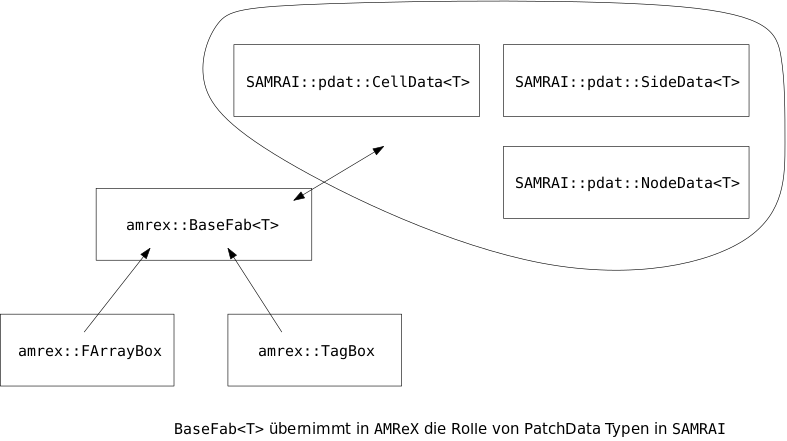
\includegraphics[width=\textwidth]{BaseFab}
\end{center}
\end{frame}

\begin{frame}[fragile]{Daten Verwaltung}
\begin{center}
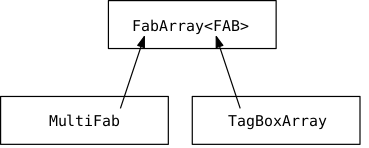
\includegraphics[width=0.5\textwidth]{MultiFab}
\end{center}

\texttt{FabArray} definiert Patch Daten für alle lokalen Boxen eines \texttt{(BoxArray, DistributionMapping)}-Paares. 
\begin{lstlisting}
// ba is amrex::BoxArray
// dm is amrex::DistributionMapping
int ncomp = 4;
int ngrow = 1;
amrex::MultiFab mf(ba, dm, ncomp, ngrow);
\end{lstlisting}
\texttt{mf} hat eine Ghost-Zellweite von 1 in jede Raumrichtung und 4 Komponenten.
\pause\\
\vspace{0.4cm}
\texttt{amrex::Geometry} entspricht der \texttt{SAMRAI::geom::CartesianGridGeometry} und wird unabhängig von den 
\texttt{MultiFabs} einer Applikation verwaltet.
\end{frame}

\begin{frame}[fragile]{Daten Verwaltung}
In \texttt{SAMRAI} ist es viel komplizierter Datenarrays für ein \texttt{BoxLevel} anzulegen! 
Das liegt an der starken Koppelung zu \texttt{SAMRAI::hier::VariableDatabase}.

\begin{lstlisting}
SAMRAI::tbox::Dimension dim(2);
int ncomp = 4;
int ngrow = 1;

// VariableDatabase is a Singleton object
SAMRAI::hier::VariableDatabase* vardb = SAMRAI::hier::VariableDatabase::GetDatabase();

// Register Cell Variable + Context with ncomp components and given ghost cell width
std::shared_ptr<SAMRAI::hier::VariableContext> context = 
    vardb->getContext("Your_Unique_Module_Context_Name");

std::shared_ptr<SAMRAI::pdat::CellVariable<double>> mass = 
    std::make_shared<SAMRAI::pdat::CellVariable<double>>(dim, "mass", ncomp);

// This line crashes the application if the variable + context pair already exists.
int mass_id = vardb->registerVariableAndContext(
    mass, context, std::vector<int>{ngrow, ngrow});

// box_level is SAMRAI::hier::BoxLevel
// geom is std::shared_ptr<BaseGridGeometry>

SAMRAI::hier::PatchLevel level(box_level, geom);
level.allocatePatchData(mass_id);
\end{lstlisting}
\end{frame}

\begin{frame}[fragile]{Gitter Generieren}
Wie werden in \texttt{AMReX} Gitter generiert?\pause\\
Durch Vererbung von \texttt{amrex::AmrCore}!
\pause
\begin{lstlisting}
//! Tag cells for refinement.  TagBoxArray tags is built on level lev grids.
virtual void ErrorEst (int lev, TagBoxArray& tags, Real time,
                       int ngrow) override = 0;

//! Make a new level from scratch using provided BoxArray and DistributionMapping.
//! Only used during initialization.
virtual void MakeNewLevelFromScratch (int lev, Real time, const BoxArray& ba,
                                      const DistributionMapping& dm) override = 0;

//! Make a new level using provided BoxArray and DistributionMapping and fill
//  with interpolated coarse level data.
virtual void MakeNewLevelFromCoarse (int lev, Real time, const BoxArray& ba,
                                     const DistributionMapping& dm) = 0;

//! Remake an existing level using provided BoxArray and DistributionMapping
//  and fill with existing fine and coarse data.
virtual void RemakeLevel (int lev, Real time, const BoxArray& ba,
                          const DistributionMapping& dm) = 0;

//! Delete level data
virtual void ClearLevel (int lev) = 0;
\end{lstlisting}
\end{frame}

\begin{frame}[fragile]{Gitter Generieren}
Wie werden in \texttt{SAMRAI} Gitter generiert?\pause\\
Durch verwendung von \texttt{SAMRAI::mesh::GriddingAlgorithm} und Vererbung von \texttt{SAMRAI::mesh::TagAndInitializeStrategy}!
\pause
\begin{lstlisting}
//! Initialize data on a new level after it is inserted into an AMR patch
//! hierarchy by the gridding algorithm.
virtual void
initializeLevelData(const std::shared_ptr<hier::PatchHierarchy>& hierarchy,
                    const int level_number, const double init_data_time,
                    const bool can_be_refined, const bool initial_time,
                    const std::shared_ptr<hier::PatchLevel>& old_level,
                    const bool allocate_data) = 0;

//! Set integer tags to "one" on the given level to identify where refinement of
//! that level should occur.
virtual void
tagCellsForRefinement(const std::shared_ptr<hier::PatchHierarchy>& hierarchy,
                      const int level_number, const int regrid_cycle,
                      const double regrid_time, const int tag_index,
                      const bool initial_time, const bool coarsest_sync_level,
                      const bool can_be_refined,
                      const double regrid_start_time) = 0;

//! After hierarchy levels have changed and data has been initialized on the new
//! levels, this routine can be used to reset any information needed by the
//! solution method that is particular to the hierarchy configuration.
virtual void resetHierarchyConfiguration(
    const std::shared_ptr<hier::PatchHierarchy>& hierarchy,
    const int coarsest_level, const int finest_level) = 0;
\end{lstlisting}
\end{frame}

\begin{frame}[fragile]{Daten Kommunikation}
In \texttt{AMReX} gibt es freie Funktionen für die Datenkommunikation von Ghost-Zellen.
\begin{lstlisting}
void FillPatchSingleLevel(MultiFab& mf, Real time, const Vector<MultiFab*>& smf,
                          const Vector<Real>& stime, int scomp, int dcomp,
                          int ncomp, const Geometry& geom,
                          PhysBCFunctBase& physbcf, int bcfcomp);

void FillPatchTwoLevels(MultiFab& mf, Real time, const Vector<MultiFab*>& cmf,
                        const Vector<Real>& ct, const Vector<MultiFab*>& fmf,
                        const Vector<Real>& ft, int scomp, int dcomp, int ncomp,
                        const Geometry& cgeom, const Geometry& fgeom,
                        PhysBCFunctBase& cbc, int cbccomp, PhysBCFunctBase& fbc,
                        int fbccomp, const IntVect& ratio, Interpolater* mapper,
                        const Vector<BCRec>& bcs, int bcscomp,
                        const InterpHook& pre_interp = NullInterpHook(),
                        const InterpHook& post_interp = NullInterpHook());
\end{lstlisting}
\end{frame}


\begin{frame}[fragile]{Daten Kommunikation}
In \texttt{SAMRAI} ist die Kommunikation in \texttt{SAMRAI::xfer::RefineAlgorithm} und \texttt{SAMRAI::xfer::RefineSchedule} geteilt.
\begin{lstlisting}
std::vector<int> data_ids{/* ... */};
std::vector<int> scratch_ids{/* ... */};
assert(data_ids.size() == scratch_ids.size());
const int n_components = data_ids.size();

// You do not need to rebuild the algorithm if a hierarchy is regrid
auto algorithm = std::make_shared<SAMRAI::xfer::RefineAlgorithm>();
for (int component = 0; component < n_components; ++component) {
  algorithm->registerRefine(
      scratch[component], data_ids[component], scratch[component],
      std::make_shared<SAMRAI::pdat::CellDoubleConstantRefine>());
}

// Whenever you change a PatchLevel you have to rebuild the RefineSchedule
std::shared_ptr<SAMRAI::hier::PatchLevel> = patch_level = hierarchy->getPatchLevel(level);
std::shared_ptr<SAMRAI::xfer::RefineSchedule> schedule =  
	algorithm->createSchedule(patch_level, level - 1, hierarchy, &boundary_condition);

// Whenever you want to fill the ghost layer
schedule->fillData(time_point);
\end{lstlisting}
\end{frame}

\begin{frame}[fragile]{Daten Kommunikation}
In \texttt{SAMRAI} scheint es auf den ersten Blick komplizierter zu sein, aber die Parameter für die freien Funktionen
\texttt{amrex::FillPatchSingleLevel} und \texttt{amrex::FillPatchTwoLevels} zu sammeln, macht auch Arbeit.
\begin{lstlisting}
void HyperbolicSplitIntegratorContext::FillGhostLayerSingleLevel(
    int level, Direction dir, BoundaryCondition boundary) {
  ::amrex::Vector<::amrex::BCRec> bcr(2 * AMREX_SPACEDIM);
  ::amrex::MultiFab& scratch = GetScratch(level, dir);
  const int nc = scratch.nComp();
  const ::amrex::Vector<::amrex::MultiFab*> smf{&GetData(level)};
  const ::amrex::Vector<double> stime{GetTimePoint(level, dir).count()};
  const ::amrex::Geometry& geom = GetGeometry(level);
  AdaptBoundaryCondition condition(boundary, geom, level);
  ::amrex::FillPatchSingleLevel(scratch, stime[0], smf, stime, 0, 0, nc, geom,
                                condition, 0);
}
\end{lstlisting}
\end{frame}

\begin{frame}[fragile]{Daten Kommunikation}
In \texttt{SAMRAI} scheint es auf den ersten Blick komplizierter zu sein, aber die Parameter für die freien Funktionen
\texttt{amrex::FillPatchSingleLevel} und \texttt{amrex::FillPatchTwoLevels} zu sammeln, macht auch Arbeit.
\begin{lstlisting}
void HyperbolicSplitIntegratorContext::FillGhostLayerTwoLevels(
    int fine, int coarse, Direction dir, BoundaryCondition boundary) {
  FUB_ASSERT(coarse >= 0 && fine > coarse);
  ::amrex::Vector<::amrex::BCRec> bcr(2 * AMREX_SPACEDIM);
  ::amrex::MultiFab& scratch = GetScratch(fine, dir);
  const int nc = scratch.nComp();
  const ::amrex::Vector<::amrex::MultiFab*> cmf{&GetData(coarse)};
  const ::amrex::Vector<::amrex::MultiFab*> fmf{&GetData(fine)};
  const ::amrex::Vector<double> ct{GetTimePoint(coarse, dir).count()};
  const ::amrex::Vector<double> ft{GetTimePoint(fine, dir).count()};
  const ::amrex::Geometry& cgeom = GetGeometry(coarse);
  const ::amrex::Geometry& fgeom = GetGeometry(fine);
  const ::amrex::IntVect ratio = 
      GetRefineRatioToCoarserLevel(fine) * ::amrex::IntVect::TheUnitVector();
  ::amrex::Interpolater* mapper = &::amrex::pc_interp;
  AdaptBoundaryCondition fine_condition(boundary, fgeom, fine);
  AdaptBoundaryCondition coarse_condition(boundary, cgeom, coarse);
  ::amrex::FillPatchTwoLevels(scratch, ft[0], cmf, ct, fmf, ft, 0, 0, nc, cgeom,
                              fgeom, coarse_condition, 0, fine_condition, 0,
                              ratio, mapper, bcr, 0);
}
\end{lstlisting}
\end{frame}

\begin{frame}[fragile]{Daten Kommunikation}
Gitterdaten werden in jedem Zeitschritt von den feineren Leveln vergröbert. In \texttt{AMReX} gibt es für diesen Zweck
verschiedene \texttt{averave\_down\_XXX} Funktionen.
\begin{lstlisting}
void HyperbolicSplitIntegratorContext::CoarsenConservatively(int fine_level,
                                                             int coarse_level,
                                                             Direction dir) {
  const int first =
      GetPatchHierarchy()->GetDataDescription().first_cons_component;
  const int size = GetPatchHierarchy()->GetDataDescription().n_cons_components;
  ::amrex::average_down(GetScratch(fine_level, dir),
                        GetScratch(coarse_level, dir), GetGeometry(fine_level),
                        GetGeometry(coarse_level), first, size, 2);
}
\end{lstlisting}
\end{frame}

\begin{frame}[fragile]{Daten Kommunikation}
In \texttt{SAMRAI} ist die Kommunikation in \texttt{SAMRAI::xfer::CoarsenAlgorithm} und \texttt{SAMRAI::xfer::CoarsenSchedule} geteilt.
\begin{lstlisting}
std::vector<int> scratch_ids{/* ... */};
std::vector<int> cons_indices{/* indices into scratch_ids */};

// You do not need to rebuild the algorithm if a hierarchy is regrid
auto algorithm = std::make_shared<SAMRAI::xfer::CoarsenAlgorithm>(dim);
for (int cons : cons_indices) {
  algorithm->registerCoarsen(
      scratch[cons], scratch[cons],
      std::make_shared<SAMRAI::geom::CartesianCellDoubleWeightedAverage>());
}

// Whenever you change a PatchLevel you have to rebuild the RefineSchedule
std::shared_ptr<SAMRAI::hier::PatchLevel> coarse = hierarchy->getPatchLevel(lvl - 1);
std::shared_ptr<SAMRAI::hier::PatchLevel> fine = hierarchy->getPatchLevel(lvl);
std::shared_ptr<SAMRAI::xfer::CoarsenSchedule> schedule = 
    algorithm.createSchedule(coarse, fine);

// Whenever you want to coarsen your data
schedule->fill(time_point);
\end{lstlisting}
\end{frame}

\end{document}